\chapter{Konzeption}\label{ch:Konzeption}

In diesem Kapitel werde ich die Konzeption hinter den Schwarmrobotern genauer beschreiben. Dazu gehört die Struktur des Systems generell, aber auch wichtige Algorithmen die die Roboter selbst, aber auch deren Interaktion mit anderen beschreiben.

\section{Generelles zur Konzeption}

Die Konzeption dieser Thesis beruht darauf, dass ROS (Robot Operating System) genutzt wird. ROS ist ein Framework, dass die Erstellung von Robotern erleichtern soll und arbeitet mit Nodes, ähnlich Microservices. Diese Nodes können als Publisher fungieren, die Nachrichten an ein Topic senden und welche man dann abonnieren kann. Sie können aber auch als Services dienen, denen man Daten sendet und von denen man anschließend eine Antwort erwarten kann.

Die Konzeption ist in 3 Phasen unterteilt, die das Konzept zum letztlichen Ziel führen werden. Der Sinn hinter diesen 3 Phasen, ist eine Iteration. Die anderen Kapitel (Implementierung und Evaluation) werden parallel geführt werden und nach jeder Phase der Konzeption wird das System zuerst prototypisch gebaut und anschließend evaluiert. Dadurch kann die Konzeption in seinen weiteren Phasen auf die Ergebnisse der vorangegangenen eingehen und auf den neuen Erkenntnissen aufbauen. Außerdem wird dadurch sichergestellt, dass das Verhalten der Roboter nicht zu sehr auf die Aufgabe des Transports zugeschnitten wird. Das ist deswegen wichtig, weil das zugrundeliegende System ein natürliches Schwarmverhalten, ähnlich dem von Tieren, sein soll und keine Gruppe von autonomen, aber strategisch denkenden Robotern.

\section{Nachbau des Schwarms nach Craig Reynolds}
Da der Transport des Schwarms auf den 3 (bzw. 4) Grundregeln des Schwarmverhaltens besteht, welche von Craig Reynolds erstmals modelliert wurden\cite{CraigReynolds_Boids}, galt es diese erst nachzustellen und zu analysieren. Reynolds selbst stellte nur die ersten drei Regeln auf. Eine vierte wurde hinzugefügt, da diese im realen Einsatz Sinn macht und auch im natürlichen Verhalten von Tieren zu sehen ist. Der Schwarm wurde zunächst nachgebaut, ohne auf die spätere Verwendung für Transporte zu achten, da diese (möglichst) ohne Kompromisse auf dem Schwarm-Prinzip aufbauen sollten. 

\subsection*{Ziel}

Das Ziel der ersten Phase ist es, grundsätzliches Schwarmverhalten nachzubauen und dieses zu messen. Es werden individuelle Roboter erstellt, die sich nur dadurch bewegen, indem sie sich an anderen Einheiten orientieren und dabei noch ihren freien Willen in die Entscheidung der Bewegungsrichtung einfließen lassen. Anschließend wird gemessen, auf welche Weise die verschiedenen Parameter das Verhalten der Roboter beeinflussen.

\subsection*{Messages}\label{subsec:NachbauNachrichten}

Die Roboter brauchen einige Informationen über die anderen Roboter, darunter vor allem die Positionen und Ausrichtungen derer, die innerhalb einer bestimmten Reichweite liegen. Diese Informationen könnten über Sensoren kommen. Da diese Sensoren aber ungenau und kostspielig sind, wird davon ausgegangen, dass sie in der Praxis nicht zur Verfügung stehen. Die Roboter müssen ihre eigene Position stets kennen und werden daher diese Informationen direkt mit den anderen Robotern teilen.

Da der \ac{ROS}-Master als Nameserver innerhalb des Systems dient, ist zu diesem eine ständige Verbindung notwendig. Dieser kann aber auf einem normalen Roboter gestartet werden. Es ist also keine weitere Einheit notwendig, wodurch das Gesamt-System homogener bleibt, wenn auch immer eine direkte Verbindung zum Master bestehen bleiben muss. Es gibt Bemühungen \ac{ROS} für mehrere, parallel laufende, Master-Nodes zu öffnen, bisher sind die Packages aber noch in der Entwicklung und es muss auf einem zentralen Master aufgebaut werden\footnote{\url{http://wiki.ros.org/multimaster_fkie}}.
Jedem Roboter wird zudem eine eindeutige ID zugewiesen werden, die es erlaubt ihn von den anderen unterscheiden zu können.

Für eine einfache Schwarm-Simulation ist nur eine Art von Nachricht notwendig. Diese enthält die Position, Ausrichtung und die ID der Roboter und wird nach jedem ausgeführten Bewegungs-Befehl gesendet. Um das System der Roboter einfacher zu halten, abonnieren die Roboter auch die Bewegungs-Daten von sich selbst. Dadurch ist es nicht notwendig diese gesondert zu behalten, sondern die Daten werden in das eigene System eingepflegt, wie die von allen anderen Einheiten auch. Möchte ein Roboter dann auf die eigenen Daten zugreifen, kennt er seine eigene ID und weiß daher welche Daten seine eigenen sind.

\subsubsection*{Neue Nachricht}
Der bisher einzig genutzte Nachrichten-Typ beinhaltet somit die Positionsdaten der einzelnen Roboter, zusammen mit der ID, wem die Daten gehören. Für die Deklaration der Nachrichten-Typen werden die Datentypen genutzt die \ac{ROS} beinhaltet\cite{ROS_MSG}. Dies erleichtert die Implementierung und die Namen der Datentypen sind außerdem selbsterklärend.

\begin{lstlisting}[style=ros, title=Nachrichten-Typ: Robot\_Position.msg]
	uint8	robot_id	// Zur Identifizierung des Absenders
	float32 pos_x		// Position des Roboters entlang der X-Achse
	float32 pos_y		// Position des Roboters entlang der Y-Achse
	float32 angle		// Ausrichtung des Roboters im Winkel von [0, 360] Grad
\end{lstlisting}

Diese Art von Nachricht wird auch den Großteil der gesendeten Nachrichten ausmachen. Das Verhalten der Roboter wird überwiegend von den Positionen anderer gesteuert, deshalb sollte dieser Nachrichten-Typ so oft wie möglich gesendet werden. Da dieser Nachricht-Typ aber auch von allen Robotern empfangen wird, beträgt die Anzahl der Nachrichten die bei der Aktualisierung des gesamten Schwarms durch das Netzwerk gehen \highlight{O(n²)}. Damit das Netzwerk nicht überfordert wird, muss deshalb ein Mittelwert gefunden werden. Zu viele Nachrichten verstopfen das Netzwerk, bei zu wenigen ist die Aktualisierung zu langsam und Roboter stoßen eventuell zusammen, weil sie die Position der anderen Roboter woanders vermuten.

\subsection*{Einhalten der 4 Grundregeln}
Die Roboter werden als autonome Einheiten konzipiert, die sich ausschließlich anhand von 3 fixen Parametern bewegen und dabei versuchen die 4 Grundregeln des Schwarmverhaltens einzuhalten. Nachfolgend werden diese vorgestellt.

\subsubsection*{Ausrichtung: Passe deine Bewegungsrichtung deinen Nachbarn an}

\begin{wrapfigure}{r}{\pictureWidth}
	\includegraphics[width=\pictureWidth,keepaspectratio]{graphics/Winkel_badCalculation.png}
	\caption{Winkel-Übersicht}
	\label{pic:Winkel_badCalculation}
\end{wrapfigure}

Da ein Roboter die Position und Ausrichtung jedes anderen Roboters kennt, ist es ohne weiteres möglich die durchschnittliche Ausrichtung der Nachbarschaft zu ermitteln. Dafür wird die Liste der Roboter genommen und die Roboter, die Nahe genug ist um relevant zu sein, in eine neue Liste kopiert. Von diesen Robotern wird dann der Durchschnitt des Winkels berechnet. Der einfache Durchschnitt, über die Summe mehrerer Winkel, würde jedoch zu einem mathematischen Schnitt führen, statt zu einem, der in der Praxis relevant ist. Daher müssen die Winkel für die Berechnung zunächst in Vektoren umgerechnet werden. Diese Vektoren werden dann addiert und der resultierende Gesamtvektor wird letztlich wieder in einen Winkel zurück gerechnet. Bei zwei gegenüberliegenden Winkeln müsste ein Roboter, der sich danach ausrichten muss, theoretisch still stehen, da die Winkel sich gegenseitig aufheben. In diesem Fall entscheidet schlicht die Ungenauigkeit der Gleitkomma-Zahlen darüber, ob er den Winkel in die eine oder in die andere Richtung nimmt.

\paragraph*{Beispiel: Fehlerhafte Winkel-Berechnung}
\autoref{pic:Winkel_badCalculation} zeigt ein Beispiel für einen Fehler, beim Berechnen des Durchschnitts zweier Winkel. Zwei Roboter mit den Winkeln 45° und 315° würden zu einem durchschnittlichen Winkel von 180° führen. Der richtige Winkel in Anbetracht der Ausrichtung wäre jedoch 0°.
 
\subsubsection*{Zusammenhang: Versuche deinen Nachbarn nahe zu sein}

%\begin{wrapfigure}{r}{\pictureWidthBig}
%	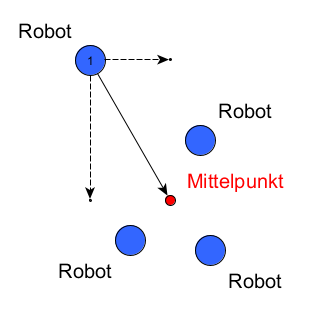
\includegraphics[width=\pictureWidthBig,keepaspectratio]{graphics/SchwarmMittelpunktBerechnung.png}
%	\caption{Berechnung des Mittelpunkts}
%	\label{pic:BerechnungMittelpunkt}
%\end{wrapfigure}

Dieser Abschnitt wird realisiert, indem zuerst die Liste der Roboter, die nahe genug sind um zur Nachbarschaft zu gehören, wieder hergenommen wird. Anschließend wird ein simpler Durchschnitt über alle Positionen (x/y - Koordinaten), der vorhandenen Roboter berechnet. Die resultierenden Koordinaten werden von den eigenen Koordinaten abgezogen, um die relative Position des Schwarm-Mittelpunkts zu bekommen. Indem man nun die relativen Koordinaten als Vektor behandelt und dadurch zu einem Winkel umrechnet, erhält man letztlich den relativen Winkel, den der Roboter anfahren müsste um zum Mittelpunkt seines Schwarms zu gelangen. Dieser Winkel wird mit normaler Geschwindigkeit angefahren.

\paragraph*{Design-Entscheidung: Mittelpunkt des Schwarms}
Um den Mittelpunkt des Schwarms zu berechnen, können verschiedene Algorithmen verwendet werden. Die einfachste Wahl, wäre der Mittelpunkt über die Koordinaten, den die (bis zu 4) äußersten Roboter im Koordinaten-System aufspannen. Dieser Mittelpunkt wäre sehr schnell zu berechnen, bezieht aber nicht mit ein, wie die Roboter innerhalb dieser Fläche verteilt sind.
Eine andere Wahl wäre der geometrische Schwerpunkt der konvexen Hülle, den die Roboter in ihrer Formation aufspannen. Dieser Mittelpunkt wäre etwas genauer in Hinblick auf die konkrete Form. Aber auch hier würde nicht die tatsächliche Verteilung beachtet werden, wenn auch genauer als in der vorigen Methode.

Eine sehr einfache Methode um die einzelnen Roboter innerhalb der Formation besser gewichten zu können, ist ein normaler Durchschnitt über die Summe der Koordinaten der einzelnen Roboter. Diese Methode verbraucht wenig Ressourcen, fast keine Kenntnisse bei der Implementierung und bietet theoretisch auch die Möglichkeit einzelne Roboter stärker zu gewichten als andere, falls dies später sinnvoll wäre. Da diese Methode sowohl die schnellste, die genauste, als auch die flexibelste ist, wurde sich für diese entschieden.

\begin{figure}[h]
	\centering
	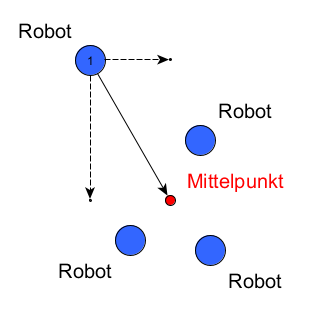
\includegraphics[width=0.8\textwidth,keepaspectratio]{graphics/SchwarmMittelpunktBerechnung.png}
	\caption{Berechnung des Mittelpunkts}
	\label{pic:BerechnungMittelpunkt}
\end{figure}

\autoref{pic:BerechnungMittelpunkt} zeigt eine Darstellung, wie der Mittelpunkt in einem Schwarm mit mehreren Roboter angelegt ist.
Die Roboter zieht es dadurch eher zu Gruppen anderer Roboter als zu Einzelgängern. Würde es den Roboter zur Mitte der konvexen Hülle ziehen, wäre die Gefahr groß, dass er alle Roboter verlieren würde, da sie zu allen Seiten gleich weit entfernt sind. Durch die einfache Methode des Mittelwerts bleibt der Roboter stets näher an Gruppen und lässt notfalls einzelne Roboter ziehen um die Gruppe zu behalten.

\subsubsection*{Abschottung: Vermeide Kollisionen mit deinen Nachbarn}

Bevor ein Roboter seinen Bewegungs-Befehl ausführt, wird mit den gewünschten Parametern eine interne Simulation durchgeführt, um die Roboter vor Kollisionen zu bewahren. Außerdem müssen sie eine Größe und eine Fläche (in einer 2dim Simulation) erhalten. Während der Simulation wird getestet, ob der gewünschte Winkel im Zusammenhang mit der Geschwindigkeit zu einer Kollision mit anderen Robotern führen würde. Eine Bewegung wird als gültig befunden, wenn der Roboter an seinem Zielpunkt mindestens seine Größe als Abstand zu allen anderen Robotern hat. Praktisch wurde die Größe um 10\per erweitert, um eine gewisse Fehlertoleranz zu erlauben.
Auch die Frequenz, der in \autoref{subsec:NachbauNachrichten} erwähnten Positions-Nachrichten, spielt hier wieder eine Rolle. 2 Roboter können dann aufeinander zufahren, wenn der Abstand beider Roboter nicht innerhalb der nächsten Aktualisierung der Positionsdaten überwunden werden kann.

\begin{wrapfigure}{r}{\pictureWidth}
	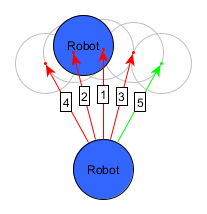
\includegraphics[width=\pictureWidth,keepaspectratio]{graphics/AusweichenAlgorithmus.png}
	\caption{Ausweichen gegenüber Hindernissen}
	\label{pic:AusweichenAlgorithmus}
\end{wrapfigure}

Ob eine Kollision am Ziel (oder unterwegs) stattfinden wird, wird mittels interner Simulationen überprüft, die die letzten Positionsdaten der Roboter nutzt.
Findet eine Kollision statt, prüft der Roboter Ausweichmöglichkeiten. Der Algorithmus wird dabei angewendet, egal ob das Hindernis ein anderer Roboter ist oder eine Gefahrenzone. Ist der Weg geradeaus nicht möglich, wird abwechselnd versucht nach links und rechts auszuweichen, wie in~\autoref{pic:AusweichenAlgorithmus} gezeigt wird. Dabei wird der Winkel, der zum Ausweichen genutzt wird, stufenweise erhöht, bis man letztlich 180° zu beiden Seiten erreicht hat, was einem Schritt rückwärts entspricht. Führt auch dieser letzte Winkel nicht zu einem erfolgreichen Ergebnis, wird der Algorithmus erneut mit einer leicht geringeren Geschwindigkeit (was ebenfalls einer leicht geringeren Bewegungsdistanz entspricht) gestartet. Erst wenn eine Simulation eine erfolgreiche Bewegung generieren konnte, wird diese auch ausgeführt.

\subsubsection*{Flucht: Fliehe vor Dingen, die eine potentielle Gefahr darstellen}

Gefahren wie Hindernisse, Löcher im Boden oder Zonen mit sich bewegenden Maschinen können die Roboter beschädigen, weshalb es gilt diesen auszuweichen. Bei jeder Bewegung muss geprüft werden, ob man mit der angestrebten Bewegung eine Gefahrenzone betreten würde. Wenn ja, wird versucht mit dem Algorithmus des vorigen Abschnitts auszuweichen.

Um Gefahrenzonen abbilden zu können, werden Objekte erzeugt die sich aus verschiedenen Geometrien, mitsamt Positionen, zusammensetzen. Betritt ein Roboter eine der im Objekt inne liegenden Geometrien, ist das Objekt als ganzes betreten worden und der Roboter befindet sich in einer Gefahrenzone.

\paragraph*{Design-Entscheidung: Abbildung von Objekten}
Um ein Objekt zu definieren ließen sich auch andere Methoden nutzen. Punkte die die Zone umspannen und eine konvexe Hülle bilden oder der Reihenfolge nach mit Geraden verbunden werden, wären ebenfalls eine Option. Allerdings wären diese viel komplexer zu berechnen und es würde mehr Rechenleistung verbrauchen.
Auch Funktionen, aus denen sich die einzelnen Punkte heraus berechnen lassen, wären denkbar um Objekte darzustellen. Um diese aber zu verteilen, müsste sie aber in einer Syntax hinterlegt werden die sich serialisieren lässt und anschließend interpretiert werden. Außerdem wären die Funktionen kompliziert zu erstellen, wohingegen ein paar Geometrien schnell abgemessen sind.

Die Berechnung, ob sich ein geometrischen Objekt innerhalb eines anderen geometrischen Objektes befindet, ist allerdings ein häufiges und gut gelöstes Problem von Videospielen\cite{GamingCollision}, weswegen diese Lösung als die beste angesehen wurde.

\subsection*{Parameter der Bewegung}

Konfiguriert wird das Schwarmverhalten der Roboter allgemein durch 4 Parameter, die in den nachfolgenden Abschnitten näher erläutert werden.

%\begin{wrapfigure}{r}{\pictureWidthBig}
%	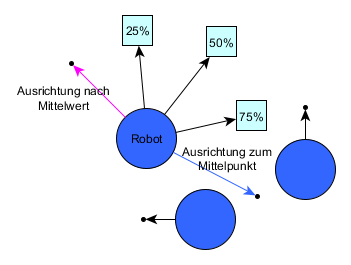
\includegraphics[width=\pictureWidthBig,keepaspectratio]{graphics/BerechnungDrangZurGruppe.png}
%	\caption{Berechnung des Drangs zur Gruppierung}
%	\label{pic:BerechnungDrangZurGruppe}
%\end{wrapfigure}

\paragraph*{Geschwindigkeit} Die Geschwindigkeit gibt an, wie schnell ein Roboter sich bewegt. Ein kleinerer Wert sorgt für langsamere, aber auch 'vorsichtigere' Roboter. Optimal wäre ein kleiner Wert in Geschwindigkeit, aber eine hohe Frequenz an Bewegungs-Befehlen.

\paragraph*{Lokale Reichweite} Da ein Roboter nur seine unmittelbare Umgebung imitiert, braucht es dafür einen Grenzwert. In dieser Thesis wurde sich für eine Begrenzung in der Reichweite (im Gegensatz zu einer Begrenzung in der Anzahl der ausgewählten Roboter) entschieden. Für die Orientierung wurde mehr Wert auf die örtliche Reichweite gelegt, da die unmittelbare Umgebung wichtiger ist, als eine feste Anzahl an Robotern an denen sich orientiert wird. Einheiten die weiter entfernt sind als dieser Wert (in der entsprechenden Maßeinheit), werden für Berechnungen ignoriert. Ein Wert kleinerer als die eigene physikalische Größe, führt zwangsläufig dazu, dass die Roboter nur sich selbst beachten.

\paragraph*{Nähe zum Schwarm} Dieser Wert ist verbunden mit der Regel 'Zusammenhang: Versuche deinen Nachbarn Nahe zu sein'. Ein Roboter hat den Drang seinem Schwarm nahe zu bleiben und versucht sich, bis zu einem gewissen Grad, in dessen Richtung zu bewegen. Da der Drang zum Schwarm nahe zu bleiben als Teil des freien Willens betrachtet wird, wird dieser Wert prozentual angegeben und nach dem freien Willen auf den endgültigen Winkel aufgerechnet. Wie genau der Drang zur Gruppierung in Prozente eingeteilt ist, wird in \autoref{pic:BerechnungDrangZurGruppe} skizziert dargestellt.

\begin{figure}[h]
	\centering
	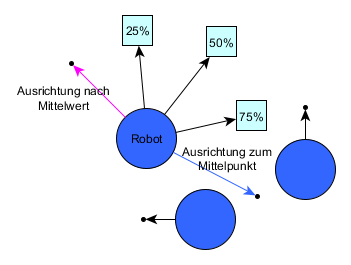
\includegraphics[width=0.7\textwidth,keepaspectratio]{graphics/BerechnungDrangZurGruppe.png}
	\caption{Berechnung des Drangs zur Gruppierung}
	\label{pic:BerechnungDrangZurGruppe}
\end{figure}

Der pinke Pfeil stellt die Richtung dar, in der sich der Roboter bei keinem Gruppendrang bewegen würde. Der blaue Pfeil ist die Richtung zum Mittelpunkt des Schwarms, diesen Weg würde er bei 100\per Gruppendrang fahren. Die anderen Pfeile wären die Richtungen bei den jeweiligen Prozentwerten.

\paragraph*{Freier Wille} Einheiten im Schwarm orientieren sich nicht nur an ihren Nachbarn, sondern besitzen in gewisser Weise auch einen eigenen Willen. Nachdem die Berechnung der Orientierung am Schwarm abgeschlossen ist, wird der eigene Wille einberechnet. Bei einem freien Willen von x°, wird dieser zufällig zwischen [-x/2, x/2] ausgesucht und dem bisherigen Winkel aufgerechnet wird. Der freie Wille ist der Parameter der mich am meisten das generelle Verhalten des Schwarms beeinflusst. Er entscheidet darüber, wie viel Zufall in der Bewegung des Schwarms enthalten ist und wie viel sie von ihrem 'erzwungenen' Verhalten abweichen dürfen.

\subsection*{Beispiel: Berechnung einer Bewegung}

%\begin{wrapfigure}{r}{\pictureWidthBig}
%	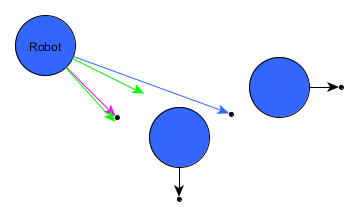
\includegraphics[width=\pictureWidthBig,keepaspectratio]{graphics/BerechnungBewegung.png}
%	\caption{Berechnung einer Bewegung}
%	\label{pic:BerechnungBewegung}
%\end{wrapfigure}

In~\autoref{pic:BerechnungBewegung} ist die Berechnung einer Bewegung skizziert. Die Pfeile geben dabei nur Richtungen an und sind nicht als Vektoren zu verstehen, die eine Aussage über die bewegte Entfernung treffen.

\begin{figure}[h]
	\centering
	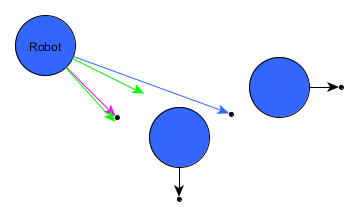
\includegraphics[width=0.6\textwidth,keepaspectratio]{graphics/BerechnungBewegung.png}
	\caption{Berechnung einer Bewegung}
	\label{pic:BerechnungBewegung}
\end{figure}

Der pinke Pfeil ist das Resultat der Berechnung des Mittelwerts der Winkel, den die anderen Roboter beim letzten Update ihrer Position haben.

Der blaue Pfeil ist der Mittelpunkt des Schwarms (in diesem Fall sind beide Roboter ein Teil der Nachbarschaft), auf den der Roboter sich aufgrund seiner Gruppenzugehörigkeit zubewegen möchte.

Die beiden grünen Pfeile sind letztlich die obere und untere Grenze des Spielraums, den der Roboter durch seinen eigenen freien Willen bekommt. Dieser wurde durch die Ausrichtung zum Schwarm-Mittelpunkt zusätzlich leicht verschoben. Aus diesen beiden Grenzen wird letztlich ein Winkel zufällig bestimmt und anschließend auf Gültigkeit (fehlende Kollisionen) geprüft, um dann schlussendlich ausgeführt zu werden.



\section{Anführer}

Um später Transportaufträge erledigen zu können, muss der Schwarm in irgendeiner Form gesteuert werden können. Bei einer direkten Steuerung aller Einheiten des Schwarms, wäre das Schwarmverhalten allerdings außer Kraft gesetzt und man hätte schlicht eine Menge gelenkter Roboter. Deswegen wurden Mittel gesucht den Schwarm indirekt zu lenken und fand diese Methode in einem Paper in dem beschrieben wurde, wie ein Schwarm über 'eingeweihte Anführer' gesteuert werden kann.\cite{VicsekLeader2}

\subsection*{Funktionsweise}
Der Anführer bietet eine passive Möglichkeit einen Schwarm zu lenken, ohne dass die normalen Einheiten angepasst werden müssen oder in ihrem Verhalten speziell abweichen müssen. Die normalen Einheiten müssen dadurch nicht wissen, dass sie ein bestimmtes Ziel haben, es muss ihnen nicht einmal bewusst sein, dass sie passiv gesteuert werden. Dadurch, dass der Anführer weiß in welche Richtung der Schwarm am besten gelenkt werden sollte, aber auch aufgrund des Gruppendrangs durch die Nachbarn, pendeln sich die anderen Einheiten des Schwarms langsam auf das Ziel ein. Ein Anführer ist somit eine Art Leuchtturm, der permanent eine Richtung angibt, ohne sich von der Umwelt beeinflussen zu lassen und der den anderen Robotern eine Orientierung gibt, ohne dass diese davon etwas mitbekommen.

Als Anführer versucht die entsprechende Einheit außerdem den Kontakt zu seinem Schwarm nicht zu verlieren. Damit ist nicht nur der Drang gemeint die Gruppenmitte aufzusuchen, der vom Anführer sowieso ignoriert wird. Es ist eine bewusstere Art auf den eigenen Schwarm acht zu geben und sich so zu bewegen, dass er weder die Gruppe verliert, noch diese ihre Ausrichtung zum Ziel zu sehr verändert. Dies ist wichtig, damit immer möglichst viele Roboter des Schwarms von der Ausrichtung des Anführers beeinflusst werden.

\subsection*{Ziel}

Ziel dieser Phase ist es, den Schwarm von einem Ort zu einem anderen zu lenken, ohne ihn wissen zu lassen, dass er gelenkt wird und möglichst ohne Einheiten auf dem Weg dorthin zu verlieren. Dies soll mit Hilfe von (möglichst wenigen) Anführer geschehen, die über das Ziel Bescheid wissen. Auf diese Weise muss in das ursprüngliche Verhalten der Roboter nicht eingegriffen werden und die Verhaltensweise der Roboter, die nicht zum Anführer erwählt wurden, bleibt exakt so bestehen wie es in der vorherigen Phase konzipiert wurde.

\subsection*{Einbindung des Anführers in ROS}

Der Anführer wurde umgesetzt, indem einer normalen Einheit ein Ziel gegeben wird und diese damit beginnt seinen Schwarm an einen bestimmten Ort zu lenken. Dazu werden die Roboter ein neues Topic abonnieren. Wenn ein Roboter diese Nachricht erhält, prüft er ob die darin enthaltene ID seiner eigenen entspricht und wenn ja, wird er den Auftrag annehmen, in den 'Anführer-Modus' wechseln und versuchen seinen Schwarm zu dem definierten Ziel zu führen. Roboter auf die ID nicht zutrifft werden die Nachricht komplett ignorieren und mit ihrem bisherigen Verhalten fortfahren.

\subsubsection*{Neue Nachricht}

Um den Transport einzuleiten wird es einen neuen Nachrichten-Typ geben. Die Nachricht kann an den Schwarm raus gesendet werden und durch die eindeutige ID weiß der entsprechende Roboter, dass er als Anführer ausgewählt wurde.

\begin{lstlisting}[style=ros, title=Nachrichten-Typ: New\_Mission.msg]
	uint8	leader_id	// Die ID des ausgewaehlten Anfuehrers
	float32 pos_x		// Position des Ziels entlang der X-Achse
	float32 pos_y		// Position des Ziels entlang der Y-Achse
\end{lstlisting}

\newpage\subsection*{Generelles Verhalten}

\begin{wrapfigure}{r}{\pictureWidthSmall}
	\includegraphics[width=\pictureWidthSmall,keepaspectratio]{graphics/AlgorithmusAnführer.png}
	\caption{Entfernungen des Anführers}
	\label{pic:AnführerReichweiten}
\end{wrapfigure}

Der Anführer steuert direkt auf das vorgegebene Ziel zu und wartet gegebenenfalls, wenn er sich zu weit vom eigenen Schwarm entfernt. Ab einer Entfernung von 75\per, der lokalen Reichweite zum Mittelpunkt seiner Herde, bleibt er stehen, bis er wieder bei 50\per Entfernung angekommen ist. Anschließend setzt er seinen Weg normal fort. Ausweichmanöver würden dafür sorgen, dass der Anführer nicht mehr auf das Ziel zeigt und damit auch die anderen Roboter dazu bringen der neuen Ausrichtung zu folgen. Aus diesem Grund wird anderen Robotern nicht ausgewichen, wie es für Schwarmroboter üblich ist. Stattdessen wird der Anführer seine Geschwindigkeit verlangsamen, wenn er mit der normalen Geschwindigkeit eine Kollision verursachen würde. Kann er sich, trotz geringerer Geschwindigkeit nicht bewegen, bleibt er stehen und wartet eine kleine Zeitspanne ab.



\subsubsection*{Einfangen eines verlorenen Schwarms}\label{subsubsec:AnführerEinfangen}
Sollte der Schwarm den Grenzbereich der lokalen Reichweite ganz verlassen, wäre es außerdem möglich, den Anführer seinen Schwarm wieder einfangen zu lassen. Dies ist in \autoref{pic:AnführerEinfangen} dargestellt.

\begin{figure}[h]
	\centering
	\includegraphics[width=0.8\textwidth,keepaspectratio]{graphics/AlgorithmusAnführerEinfangen.png}
	\caption{Anführer fängt seinen Schwarm wieder ein}
	\label{pic:AnführerEinfangen}
\end{figure}

Im ersten Abschnitt ist der Schwarm verloren gegangen, obwohl der Anführer gewartet hat. Anschließend ist er mit erhöhter Geschwindigkeit hinter den Schwarm gefahren, sodass der Schwarm sich nun genau zwischen Ziel und Anführer befindet. Nun nimmt er wieder sein normales Verhalten an und versucht den Schwarm in die Richtung des Ziel zu lenken. Beim umdrehen, um den Schwarm wieder einzufangen, dreht sich der Anführer allerdings in die entgegengesetzte Richtung. Die anderen Roboter wissen nichts von einem Manöver und orientieren sich normal am Anführer. Das kann dazu führen, dass der Schwarm zunächst noch weiter abgelenkt wird. Aus diesem Grund sollte das Einfangen so schnell wie möglich beendet werden. Die Geschwindigkeit des Anführers sollte also möglichst hoch sein.

%\begin{wrapfigure}{r}{\pictureWidthBig}
%	\includegraphics[width=\pictureWidthBig,keepaspectratio]{graphics/AlgorithmusAnführerEinfangen.png}
%	\caption{Anführer fängt seinen Schwarm wieder ein}
%	\label{pic:AnführerEinfangen}
%\end{wrapfigure}







\section{Transport von Waren mit Hilfe eines Schwarms}

Das letztliche Ziel dieser Arbeit ist es zu prüfen, ob es möglich, und sinnvoll, ist Gegenstände mit Hilfe eines autonomen Schwarms zu transportieren. Dazu musste der Schwarm nun dazu gebracht werden Waren zu bewegen, ohne die einzelnen Roboter zu sehr zu beeinflussen. Da generell die Roboter nicht zentral gesteuert werden sollen und auch die Logik möglichst simple bleiben soll, sollte das Programm der einzelnen Einheiten möglichst wenig verändert werden und der 'natürliche' Trieb der Einheiten genutzt werden.

\subsection*{Erteilen von Aufträgen}

Eine der ersten Dinge im Ablauf eines Transports ist die Erteilung des Auftrags. Um die Roboter einem bestimmten Auftrag zuzuteilen und den jeweiligen Anführern mitzuteilen, dass sie diese Rollen übernehmen müssen, braucht es neue Informationen innerhalb des \ac{ROS}-Systems. Da es den Nachrichten-Typ \highlight{New\_Mission} bereits gibt, muss dieser nur erweitert werden, sodass er nun die folgenden Felder hat:


\subsubsection*{Veränderte Nachricht}

\begin{lstlisting}[style=ros, title=Nachrichten-Typ: New\_Mission.msg]
uint8 robot_index_from		// Beginn der ID-Range
uint8 robot_index_to		// Ende der ID-Range

uint8 leader_number			// Anzahl der Leader die gebraucht werden
uint8 mission_id			// Die ID der Mission

float32 object_position_x	// Die Start-Position des Objektes, X-Achse
float32 object_position_y	// Die Start-Position des Objektes, Y-Achse

float32 object_size_x		// Die Laenge des Objektes, in X-Richtung
float32 object_size_y		// Die Laenge des Objektes, in Y-Richtung

float32 target_x			// Die Ziel-Position des Objektes, X-Achse
float32 target_y			// Die Ziel-Position des Objektes, Y-Achse
\end{lstlisting}

Der Nachrichten-Typ definiert nun eine Spanne von Robotern die den Auftrag ausführen sollen. Diese werden mit ihren IDs angesprochen. Das Intervall der IDs ist, gemäß Programmierstandards, als halboffenes Intervall definiert: [robot\_index\_from, robot\_index\_to[.

leader\_number gibt die Anzahl der Leader an die verwendet werden sollen und mission\_id gibt dem derzeitigen Auftrag eine fixe ID um diesen und zugehörige Dinge genau identifizieren und verbinden zu können. Da die Anführer den Schwarm kontrollieren müssen, werden spezielle Nachrichten notwendig sein. Um zu verhinden, dass diese von allen Anführer gesendet werden, braucht es einen 'Haupt-Anfüher'. Da der einfachste Weg ist diesen zu bestimmen, den mit der kleinsten ID zu nehmen, wird er im Folgenden entsprechend der erste Anführer genannt werden.

Mit object\_position\_x/-\_y ist die Startposition des zu transportierenden Objektes angegeben. Zusammen mit object\_size\_x/-\_y, welche die Ausmaße des Objektes angeben. Die Position des Objekts ist als Mitte des Objekts definiert.
target\_x/-\_y gibt die letztliche Position an die das Objekt einnehmen soll.

Der Auftrag wird von außen an das Topic 'flock/mission/new' gesendet. Der Ersteller des Auftrags muss keine \ac{ROS}-Node sein, auch wenn dies verschiedene Vorteile hätte. Dadurch das \ac{ROS}-Topics auch über das Terminal angesprochen werden können, ist das Senden der Nachrichten auch über jedes andere Programm möglich. Das Topic für die neuen Missionen wird von jedem aktiven Roboter abonniert. Entsprechend nimmt jeder Roboter Notiz von diesem Auftrag, auch wenn er nicht direkt mit seiner ID angesprochen wird.\\


\subsection*{Von Gefahrenzonen zu Sicherheitszonen}

Um die betreffenden Roboter in die Zone zu senden, auf der ihnen später das Transportobjekt aufgesetzt wird, wird ein Mechanismus verwendet der bereits vorher Einzug in das \ac{ROS}-System hielt: Gefahrenzonen. Diese werden leicht angepasst, um sie invertieren zu können und somit aus einer Gefahrenzone eine Sicherheitszone zu machen. Ist ein Bereich als Sicherheitszone definiert, ist jeder andere Bereich automatisch eine Gefahrenzone.
Dieser Mechanismus birgt nur eine kleine Änderung im System, schafft es aber Roboter in einen bestimmten Bereich zu locken ohne sie aktiv steuern zu müssen, indem einfach ihr 'natürlicher' Trieb verwendet wird, von Gefahren zu flüchten.

Wird ein Auftrag erteilt, so nehmen die Roboter die dem Auftrag zugeteilt sind, eine neue Sicherheitszone auf, die den Ausmaßen und der Position des Transportobjekts am Aufnahmeort entspricht. Da jeder andere Ort außerhalb der Sicherheitszone analog eine Gefahrenzone wird, werden die Roboter nun versuchen sich in diese Sicherheitszone zu bewegen. Roboter die nicht dem Transport zugeteilt wurden, werden diese neue Zone als Gefahrenzone auffassen um die Transport-Roboter nicht bei ihrer Arbeit zu stören und versuchen sich diesem Gebiet fernzuhalten.

Ein Objekt kann grundsätzlich aus verschiedenen Geometrien zusammengesetzt werden. Dadurch ist es möglich nicht nur Objekte zu transportieren die eine einfache Form wie Rechtecke oder Kreise haben, sondern verschiedene Rechtecke können dann zu einem 'L' oder 'U' zusammengesetzt werden.

\subsection*{Füllen eines Raums}

Wird eine Sicherheitszone definiert, versuchen die Roboter, die sich in der Gefahrenzone befinden, auf möglichst schnellstem Wege die Sicherheitszone zu betreten. Dazu wird der nächste, verfügbare Ort der Sicherheitszone ins Ziel genommen und (ohne mit anderen Robotern zu kollidieren) der direkte Weg darauf zu genommen. Da die Roboter sich in Gefahr denken, wird während dieser Zeit der freie Wille außer Kraft gesetzt, da das das eigene überleben den höchsten Willen eines Roboters darstellt. Die Roboter werden sich nun darin aufhalten und durch ihre zufälligen Fahrtrouten automatisch Platz für nachkommende Roboter schaffen.

\subsubsection*{Nachrichten}

Damit das Transportobjekt nun sicher auf den Robotern aufgesetzt werden kann, müssen diese nun still stehen. Ein Stillstand von Einheiten eines Schwarms ist laut den Regeln des Schwarmverhaltens nicht möglich, da es keine Regel gibt, die diesen Zustand hervorrufen könnte. Daher wird ein Trick angewendet, der weniger in das Verhalten der Roboter eingreift, als viel mehr direkt in die unteren Layer des Roboter-Systems. Bemerkt der erste Anführer, dass alle Roboter innerhalb des Transportobjektes sind, befiehlt er ihnen mit dem folgenden neuen Nachrichten-Typ still zu stehen.

\begin{lstlisting}[style=ros, title=Nachrichten-Typ: Robot\_Freeze.msg]
uint8 robot_index_from		// Beginn der ID-Range
uint8 robot_index_to		// Ende der ID-Range
\end{lstlisting}

Jeder Roboter der sich in dieser Range befindet, (egal ob er dem Auftrag zugeteilt ist oder nicht) wird daraufhin still stehen. Von hier an braucht es ein Event, dass den Robotern zeigt dass sie mit dem Transportobjekt Richtung Ziel losfahren können. Möglich wäre eine Zeitsteuerung für streng automatisierte Prozesse. Aber auch interne Signale über \ac{ROS} sind möglich. Durch die ID die jeder Auftrag hat, wäre eine einfache Nachricht '[TransportID\#][Losfahren]' bereits zielführend. Ein zweiter, neuer Nachrichten-Typ wird daraufhin die Roboter wieder aus ihrem Schlaf erwecken und sie in ihr normales Verhalten zurück werfen.

\begin{lstlisting}[style=ros, title=Nachrichten-Typ: Robot\_Continue.msg]
uint8 robot_index_from		// Beginn der ID-Range
uint8 robot_index_to		// Ende der ID-Range
\end{lstlisting}

\subsection*{Der Transport}

\begin{wrapfigure}{r}{\pictureWidthSmall}
	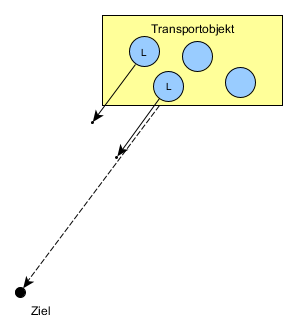
\includegraphics[width=\pictureWidthSmall,keepaspectratio]{graphics/AlgorithmusTransport.png}
	\caption{Der Transport des Objekts}
	\label{pic:AlgorithmusTransport}
\end{wrapfigure}

Um den Transport selbst zu realisieren, bedient man sich nun der Hilfe der Anführer. Diese richten sich dynamisch nach dem Winkel aus, den das Transportobjekt zum Ziel hat, wie \autoref{pic:AlgorithmusTransport} zeigt. Danach fangen sie an sich langsam in die Richtung zu bewegen in die sie sich ausgerichtet haben. Die anderen Roboter werden sich aufgrund des Gruppenverhaltens ebenfalls mehr oder weniger, gehemmt durch den eigenen freien Willen und ihrem Drang sich zur Mitte ihres Schwarms zuzubewegen, nach ihren Anführern ausrichten und das Objekt so langsam in Richtung des Ziel zu bewegen.

\subsubsection*{Einhalten der Richtung hat Priorität}

Kann ein Anführer keine normale Bewegung ausführen, weil er sonst mit einem anderen Roboter kollidieren würde, darf er nicht versuchen auszuweichen, da dies sonst die Ausrichtung der passiven Roboter negativ beeinflussen könnte. Stattdessen drosselt er zunächst sein Bewegungstempo oder bleibt, falls notwendig, ganz stehen. Die richtige Richtung beizubehalten ist wichtig, da sich passive Roboter nicht unmittelbar nach ihren Anführern ausrichten. Gerade wenn es zahlenmäßig wenige Anführer im Vergleich zu passiven Robotern sind, kann es einige Zeit dauern, bis die Einheiten so weit beeinflusst wurden, dass sie in die gewünschte Richtung zeigen. Dreht sich ein Anführer in die verkehrte Richtung, vielleicht sogar in die entgegengesetzte, kann dies zu einer Kettenreaktion führen die alle Roboter betrifft und zusätzlich das Transportobjekt stark vom Weg abbringen. Dieser Effekt konnte bereits in früheren Simulationen erkannt werden (siehe: \autoref{subsec:AnalyseNachbesserung}) und wird deshalb in dieser Phase der Konzeption vermieden.

\subsubsection*{Mitziehen des Transportobjektes}

\begin{wrapfigure}{r}{\pictureWidth}
	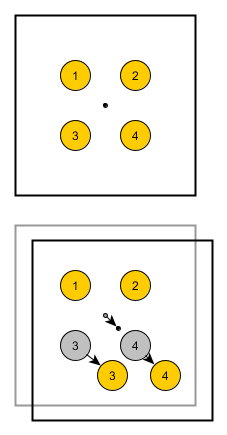
\includegraphics[width=\pictureWidth,keepaspectratio]{graphics/Transport/Tracking.png}
	\caption{Tracking des Transportobjektes}
	\label{pic:TrackingTransportobjekt}
\end{wrapfigure}

Die Roboter haben keine Sensorik, um den Zustand des physikalischen Transportobjekt zu erkennen. In der Software ist es daher als Sicherheitszone markiert. Bisher konnten Objekte in der Software allerdings nicht verschoben werden. Daher bekommen Objekte nun eine ID zugewiesen, die es ihnen erlaubt eindeutig erkannt zu werden. Außerdem müssen die Objekte nun verschoben werden können und es braucht jemanden der die Änderung des physikalischen Standorts erkennt und ihn der Software verbreitet.

Grundsätzlich gibt es für dieses Vorgehen verschiedene Vorgehensweisen. Eine davon wäre ein \ac{IPS}, das heißt ein Sensor auf dem Transportobjekt, mit einer \ac{ROS}-Node die diesen Sensor verfolgt und als Broadcast im \ac{ROS}-System verbreitet. Leider haben bisherige Erfahrungen gezeigt, dass solche \ac{IPS}s nicht sehr zuverlässig sind. Nicht nur ist die Qualität der Ortung sehr ungenau, sie springt auch zwischen den verschiedenen Messintervallen hin und her. Mehr dazu im Einschub \autoref{subsubsec:IPS}.

Um die Position des Transportobjektes im \ac{ROS}-System bekannt zu machen, und aktuell zu halten, wird deshalb darauf gesetzt, dass das Objekt auf den Robotern bleibt und diese ihre Position selbst erkennen können. Zu beginn des Transports wird die relative Position des Objektes zum Mittelpunkt des Schwarms gespeichert. Bewegt sich nun der Mittelpunkt des Schwarms in eine Richtung, wird die Position des Objektes immer relativ von diesem angesehen. Eine Verdeutlichung ist in \autoref{pic:TrackingTransportobjekt} zu sehen. Dabei werden allerdings ein paar Eingeständnisse gemacht.

\paragraph*{Zugeständnisse der Simulation}
Zum einen wird angenommen, dass die Roboter alle die selbe Reibung am Objekt haben. Würde der Transport von nur 2 Roboter erledigt werden und diese bewegten sich in entgegensetzter Richtung von einander weg, müsste das Objekt somit stillstehen. In der Realität wäre die Reibung wahrscheinlich nicht gleich, sodass das Objekt in einer Richtung abdriften würde. Es gilt aber in der Praxis festzustellen, wie viel Ungenauigkeit dadurch wirklich entstehen würde.
Eine andere Annahme wäre, dass die Reibung vom Roboter zum Objekt so hoch wäre, dass die Räder der Roboter eher stehen bleiben, statt dass der Roboter sich bewegt. Dadurch würden zwei Roboter, die in entgegengesetzter Richtung fahren, stehen bleiben. Die Roboter müssten natürlich auch erkennen, dass die Räder stehen bleiben. Da dies bei Servo-Motoren allerdings kein Problem darstellt, gilt dieser Punkt als unproblematisch.

Um die Rollenverteilung weiter einzuhalten, sollte einer der Anführer die Position des Objektes innerhalb des Schwarms aktualisieren. Dazu braucht es eine weitere, simple Nachricht.

\begin{lstlisting}[style=ros, title=Nachrichten-Typ: Update\_Object.msg]
uint8 mission_id			// Die ID der Mission

float32 object_position_x	// Die Position des Transport-Objektes, X-Achse
float32 object_position_y	// Die Position des Transport-Objektes, Y-Achse
\end{lstlisting}

Da jeder Mission nur ein Objekt zugeordnet ist und dieses, passenderweise, die ID der Mission eingetragen bekommen kann, ist es leicht möglich die Position des Objektes über die ID der Mission zu aktualisieren. Wann immer ein Roboter diesen Nachrichten-Typ empfängt, schaut er in seiner Liste nach einem Objekte mit dieser ID und setzt dessen Position auf die der Nachricht. Bei mehreren Anführern ist es grundsätzlich egal, wer die Aktualisierung sendet, es sollte aber generell bei einem Anführer bleiben, da es nicht notwendig sein sollte die Position in hoher Frequenz zu aktualisieren. Der Einfachheit halber sendet der Anführer mit der geringsten ID die Aktualisierungen. Da jeder die selbe Nachricht bekommt, wissen die anderen Roboter wer alles Anführer ist und ob sie selbst die niedrigste ID besitzen.

\paragraph*{Einschub: Unzulänglichkeiten von IPSs}\label{subsubsec:IPS}

Indoor-Positioning-Systems dienen zur Positionsbestimmung innerhalb von geschlossenen Räumen/Hallen und sind damit das kleine Äquivalent zu GPS. In vorangegangenen Tests wurde ein System eines namenhaften Hersteller getestet und für zu schlecht empfunden.

\begin{figure}[h]
	\centering
	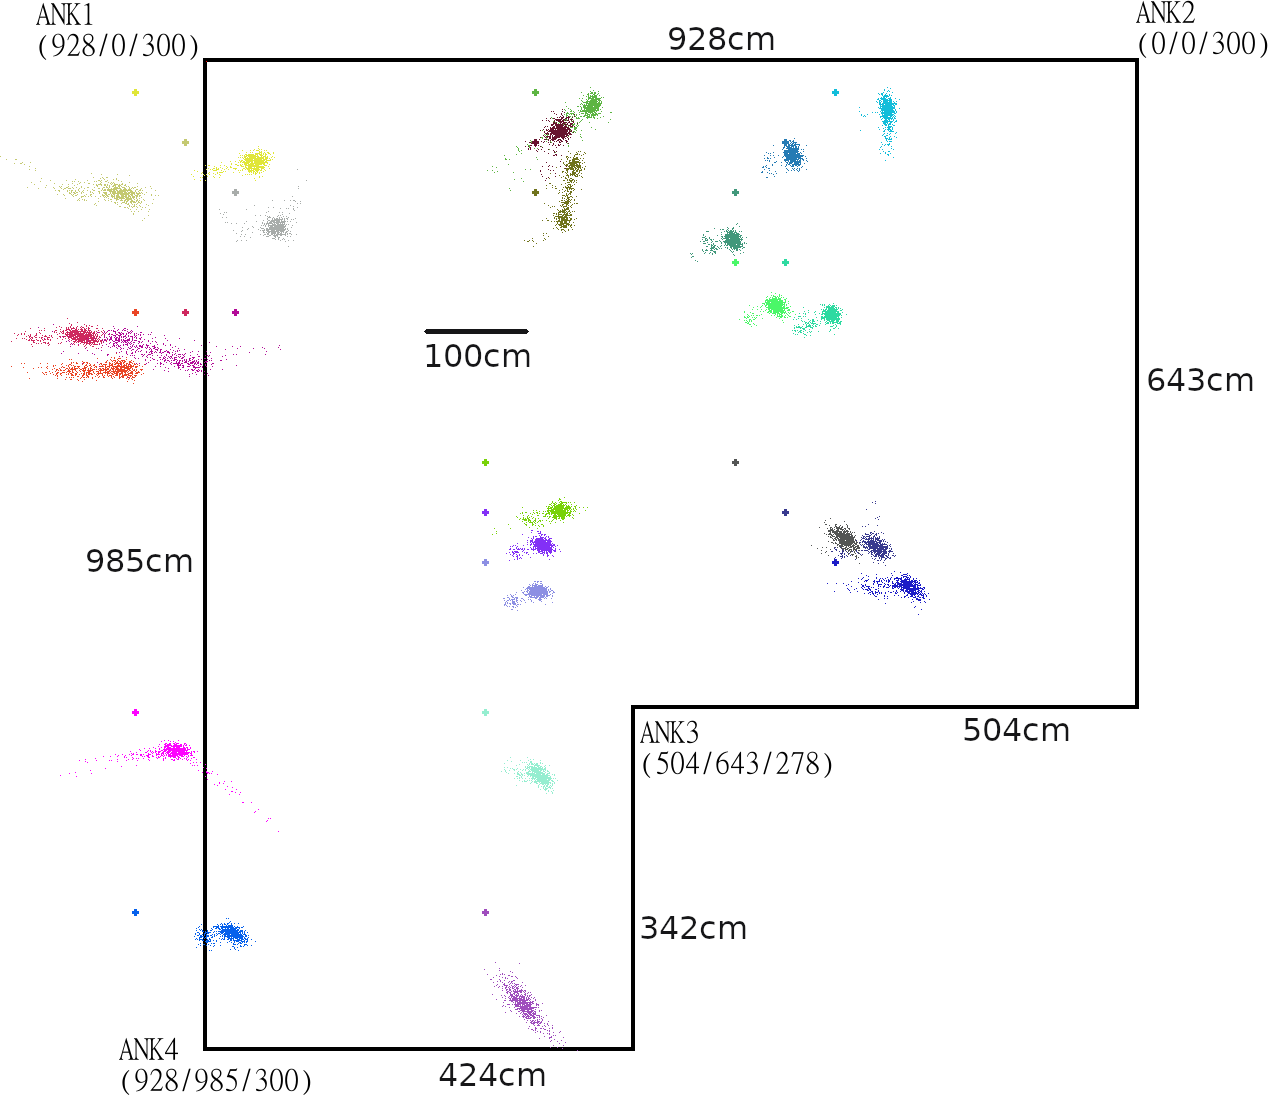
\includegraphics[width=0.8\textwidth,keepaspectratio]{graphics/Solcon/old.png}
	\caption{Evaluation eines IPS}
	\label{pic:SolconIPS}
\end{figure}

\newpage
Die Nachteile waren im groben:

\begin{itemize}
	\item Ungenauigkeiten von durchschnittlich 81cm
	\item Der Sensor muss stets Sichtkontakt zu 3 Beacons haben
	\item Der Bereich der eingegrenzt werden konnte, betrug < 100m²
\end{itemize}

%\begin{wrapfigure}{r}{\pictureWidthBig}
%	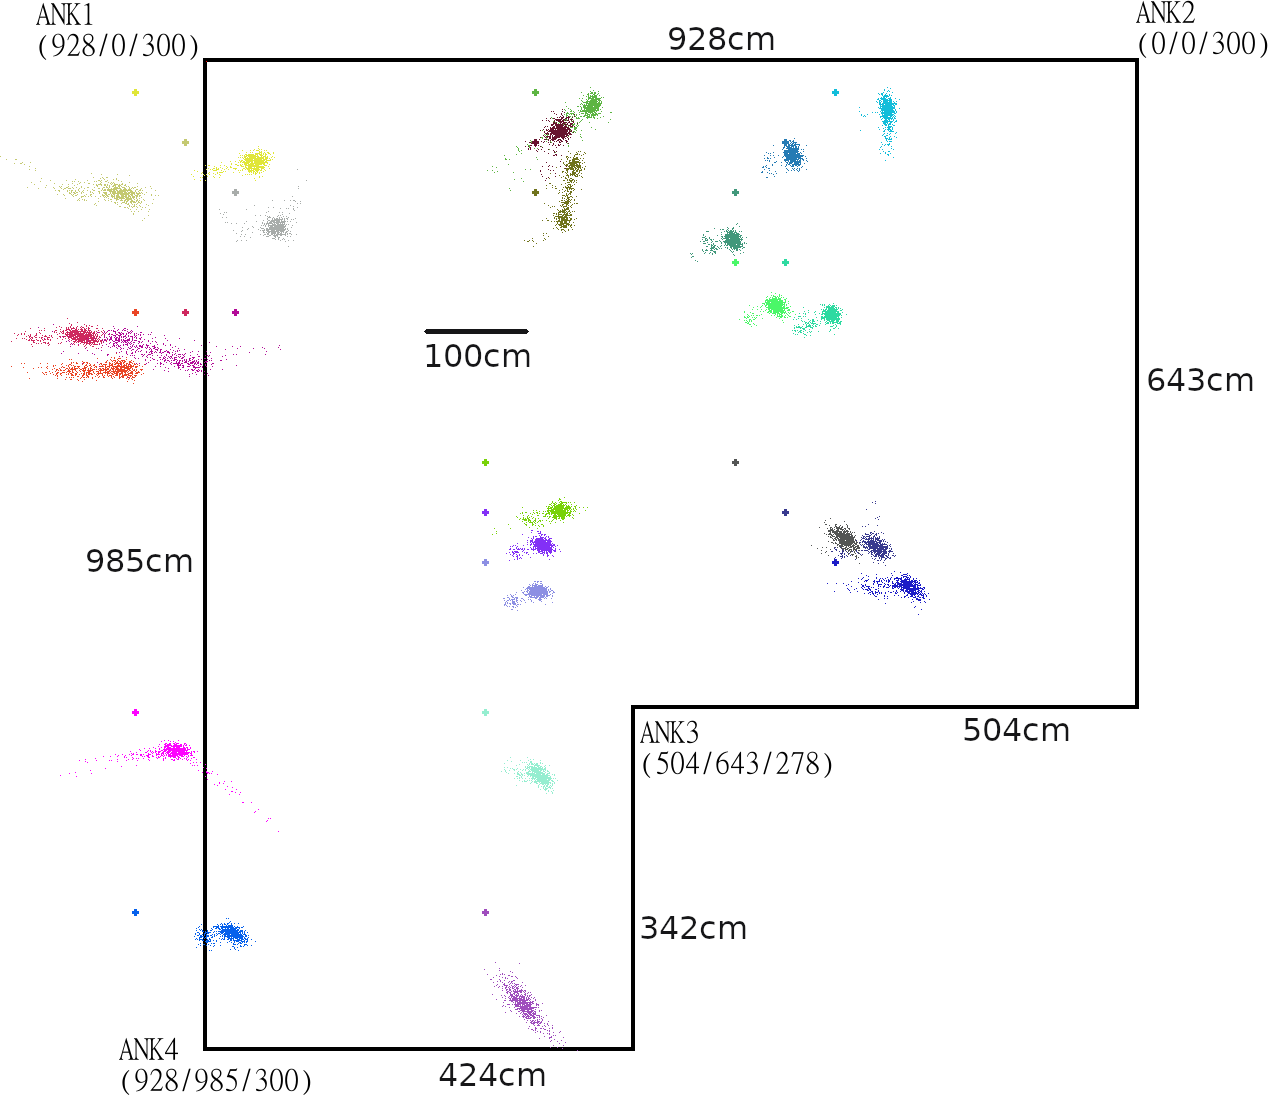
\includegraphics[width=\pictureWidthBig,keepaspectratio]{graphics/Solcon/old.png}
%	\caption{Evaluation eines IPS}
%	\label{pic:SolconIPS}
%\end{wrapfigure}

In \autoref{pic:SolconIPS} wurden Daten eines IPS in ein Bild eingetragen. Jede Farbe steht für einen anderen Testdurchlauf. Die Kreuze markieren den Punkt, an dem der Sensor, der getrackt werden sollte, tatsächlich stand. Die Punkte in selbiger Farbe sind die Standorte, an denen er laut System gemessen wurde. Abweichungen von über 1m waren eher die Regel als eine Ausnahme. Auch plötzliche Sprünge zwischen 2 Messungen (zeitlicher Abstand 100-300ms) von über 50cm waren keine Seltenheit.

Die Evaluation zeigt klar, dass solche Systeme zum aktuellen Stand noch nicht genug ausgereift, und deshalb nicht für die Ortung eines Transportobjektes geeignet, sind.

\subsection*{Abschluss des Transports}

Ist das Transportobjekt nahe genug am Ziel, ist der Transportauftrag abgeschlossen. Da die Anführer um den Mittelpunkt herum verteilt sind, kann es notwendig sein, dass einige davon selbst über das Ziel hinausschießen müssen, um den Mittelpunkt des Objektes zum Ziel zu bringen. Hier stellt sich wieder die wichtig heraus, dass sie Anführer nicht ihren Winkel zum Ziel einnehmen müssen, sondern den, den der Mittelpunkt zum Ziel hat. Hätten sie den Winkel genommen, den sie selbst zum Ziel haben, würden sie, sobald sie das Ziel erreichen, um dieses herum pendeln und den Schwarm durcheinander bringen. Dadurch, dass sie den Mittelpunkt aus Ausgangswinkel nehmen, fahren sie weiter ihrer Linie nach und das Objekt schafft es letztlich zum Ziel.

Am Ziel angekommen, sendet der erste Anführer sein letztes Update der Position und direkt danach erneut eine Nachricht vom Typ \highlight{Robot\_Freeze}, woraufhin die Roboter erneut stehen bleiben. An dieser Stelle kann, genau wie beim Aufnehmen des Transports, eine Nachricht von außen das Signal geben, dass das Objekt abgenommen wurde. Es kann, in streng gesteuerten Prozessen, aber auch ein Timer sein. Sobald das Signal kommt, wird der erste Anführer den Stillstand wieder mit einem \highlight{Robot\_Continue} aufheben und der Schwarm kehrt in seinen normalen Modus zurück. Zusätzlich muss aber noch das Transportobjekt als Hinderniss/Sicherheitszone aus dem Speicher der Roboter gelöscht werden. Dies geschieht mit dem Befehl:

\begin{lstlisting}[style=ros, title=Nachrichten-Typ: Delete\_Object.msg]
uint8 mission_id			// Die ID der Mission
\end{lstlisting}

Durch diesen Befehl, der auch für die Roboter wichtig ist, die nicht am Transport beteiligt waren, wird das Transportobjekt als Hindernis gelöscht und der Auftrag ist endgültig vorbei.












\section{Weiterführende Konzeption}

Die Implementierung der Konzeption ist prototypisch und dient vor allem dazu Statistiken erheben zu können. Durch diese Statistiken kann das Konzept in den nachfolgenden Phasen nachgebessert werden und es kann ein Gefühl dafür entwickelt werden, wie die einzelnen Parameter einen Schwarm beeinflussen, um ihn später den gegebenen Umständen besser anpassen zu können.\\

An dieser Stelle endet die prototypische Implementierung jedoch und die Konzeption wird nicht mehr nachgeprüft. Es werden Ideen vorgestellt und ausgearbeitet, wie man den Schwarm besser und dynamischer gestalten kann, die Kapitel der Implementierung und Evaluation sind dagegen beendet.

\subsection{Dynamischer Schwarm}

Der Schwarm ist bisher statisch. Man stellt eine bestimmte Anzahl an Robotern ein, aus denen der Schwarm bestehen soll und diese müssen alle gestartet werden. Fehlen Roboter oder werden zu viele gestartet, führte das bisher zu Fehlern. Neue Roboter hinzufügen oder bestehende wieder entfernen ist nicht möglich. Dies muss für einen dynamischen Schwarm geändert werden, weswegen zwei neue Nachrichten eingeführt werden die genau das erlauben.

Wird ein neuer Roboter erschaffen (oder aktiviert), stellt sich dieser mit seiner neuen ID im Schwarm vor. Die anderen Roboter im Schwarm werden diesen in ihre Liste und damit in ihre Berechnungen aufnehmen.

\begin{lstlisting}[style=ros, title=Nachrichten-Typ: New\_Robot.msg]
uint8 robot_id			// Die ID des neuen Roboters
uint8 sub_id			// Die Sub-ID des Roboters
\end{lstlisting}

\begin{lstlisting}[style=ros, title=Nachrichten-Typ: Delete\_Robot.msg]
uint8 robot_id			// Die ID des zu entfernenden Roboters
uint8 sub_id			// Die Sub-ID des Roboters
\end{lstlisting}

\subsubsection*{Einzigartigkeit gefährdet}

Mit dem dynamischen hinzufügen von Robotern kommt es jedoch zu einem weiteren Problem. Der Einzigartigkeit von IDs. Ist dies bei physischen Robotern noch gut zu kontrollieren, indem jeder Hardware eine bestimmte ID zugewiesen wird und diese in einem zentralen System kontrolliert werden. Kommt es zu Problemen, wenn Roboter virtuelle Kopien erzeugen wollen und diese neue IDs brauchen. Sind beispielsweise die IDs im Bereich von [1,10] vergeben und 2 Roboter wollen neue Kopien erzeugen, kann es zu Kollisionen kommen weil sie einer Kopie die gleiche ID zuweisen.

Natürlich könnten diese Kollisionen aufgelöst werden, beispielsweise indem man pro neuer ID die man erschafft einen Echo-Algorithmus startet und der der die Wahl gewinnt die ID bekommt. Erschafft ein Roboter aber 20 Kopien von sich kann dies sehr viele Nachrichten zur Folge haben die das Kommunikationsnetz belasten. Aus diesem Grund ist es besser Kollisionen in den ID von Anfang an zu vermeiden. Als Lösung wird die ID global im gesamten System um ein weiteres Byte erweitert, der sub\_id.

\paragraph*{Konzept: Sub-ID}
Eine sub\_id ist ein Zusatz zur normalen ID. Die robot\_id wird die Haupt-ID eines Roboters und physische Roboter werden immer unterschiedliche robot\_id's haben mit der sub\_id '0'. Möchte ein Roboter nun virtuelle Kopien von sich erstellen, erstellt er diese mit seiner robot\_id und der nächsten freien sub\_id. Auf diese Weise kann es nicht zu Kollisionen kommen, wenn mehrere Roboter gleichzeitig virtuelle Kopien erstellen. Es liegt damit außerdem in der Verantwortung der Roboter selbst ihre sub\_id's zu verwalten.





\subsection{Virtuelle Anführer}

Bisher waren die Anführer richtige Roboter, mit dem Unterschied, dass sie über das Ziel Bescheid wussten. Der nächste Schritt wäre es, die Anführer zu entkoppeln und virtuell zu machen\cite{RobotLeaderVirtual}.
Der große Vorteil eines virtuellen Anführers ist es, dass er zum einen den Schwarm nicht blockiert mit seiner Anwesenheit. Zum anderen kann eine neue Technik genutzt werden die 'Stacking' genannt wird.

\paragraph*{Stacking}
Als Stacking bezeichnet man es, mehrere Roboter übereinander zu stapeln, um ihren Einfluss zu erhöhen. Auf diese Weise nehmen n Roboter die Position und den Platz eines einzelnen Roboters ein. Dadurch kann man im Prinzip einen Roboter haben, der aber den Einfluss von n Robotern hat. Für diese Methode kann selbstverständlich nur maximal ein physischer Roboter eingesetzt werden. Die anderen die auf diesem gestackt werden, müssen virtuell sein, da deren Körper sonst zu Problemen führen würde. Natürlich kann aber auch komplett auf einen physischen Roboter verzichtet werden und es werden ausschließlich virtuelle Roboter genutzt.\\

Mit Hilfe des Stacking kann also nun ein physischer Anführer den Einfluss von n Anführern besitzen und seinen Schwarm effektiver steuern als es allein möglich wäre. Virtuelle Anführer können von einer neuen Art von Node gesteuert werden, die diese erstellt und deren Position im Schwarm pflegt oder, wenn ein physischer Anführer involviert ist, können seine physischen Kopien direkt von diesem gesteuert werden, indem er seine eigene Position mit mehreren IDs sendet. Dies setzt voraus, dass der Schwarm vorher dynamisch gemacht wurde. Dadurch kann ein Anführer nun mehrere Kopien von sich erzeugen und diese Anzahl von den beim Transport beteiligten Roboter abhängig machen.

\subsubsection*{Bewegung als virtueller Anführer}

Zwar muss ein virtuell erstellter Anführer nicht physisch aktiv sein, dennoch muss er für die anderen Roboter so aussehen als wäre er physisch aktiv und sich entsprechend bewegen. Er wird mit seinem Schwarm mitziehen müssen und darauf achten, mit niemandem zu kollidieren, da die physischen Roboter eben dies auch tun werden.

Um einen virtuellen Anführer zu erstellen, muss im Grunde genommen nur der untere Layer ausgetauscht werden, der für die Bewegung des Motors zuständig ist und der nach einer Bewegung die Positionsdaten an die höheren Layer zurück gibt.
Dieser Layer wird keinen Motor ansteuern, da die entsprechende \ac{ROS}-Node sich nicht auf einem Roboter befinden wird (oder zumindest keinem physischen Körper zugeteilt wurde). Stattdessen wird der Layer die Bewegung entgegen nehmen und die Positionsdaten zurückgeben, die bei einer perfekt ausgeführten Bewegung (ohne Rutschen oder Blockieren) zustande gekommen wären.





\subsection{Globale Statisten}

Ein anderer Ansatz um einen Schwarm zu lenken, im Gegensatz zur Nutzung eines Anführers, ist die Einführung eines still stehenden Roboters, der Statist genannt wird.

\subsubsection*{Unterschiede zum Anführer}

Ein Anführer lenkt seinen Schwarm dadurch, dass er sich innerhalb des Schwarms befindet und den Schwarm auf Grundlage der Regel 'Ausrichtung: Passe deine Bewegungsrichtung deinen Nachbarn an' (\autoref{4Rules}) manipuliert. An dieser Regel anzusetzen ist ein valider Gedanke, es gibt aber auch andere Regeln die sich manipulieren lassen. Der Statist setzt an der Regel 'Zusammenhang: Versuche einen Nachbarn nahe zu sein' an und versucht einen Schwarm dadurch zu steuern, dass die Roboter sich an der Mitte ihres Schwarms ausrichten.

\subsubsection*{Grundlage des Statisten}

Grundlage des Statisten ist es, dass er immer in die Berechnung der Schwarmmitte einbezogen wird, auch dann, wenn er sich außerhalb aller lokalen Reichweiten befindet. Er (oder vielleicht auch mehrere) werden somit einfach an den Ort setzen, an dem man den Schwarm braucht. Dadurch, dass dieser weit weg vom Schwarm positioniert wird, verzerrt er die Mitte des Schwarms entsprechend stark. Die Roboter werden nun versuchen wieder in Richtung der Schwarmmitte zu fahren und somit indirekt in die Richtung des Statisten.

%\begin{wrapfigure}{r}{\pictureWidthBig}
%	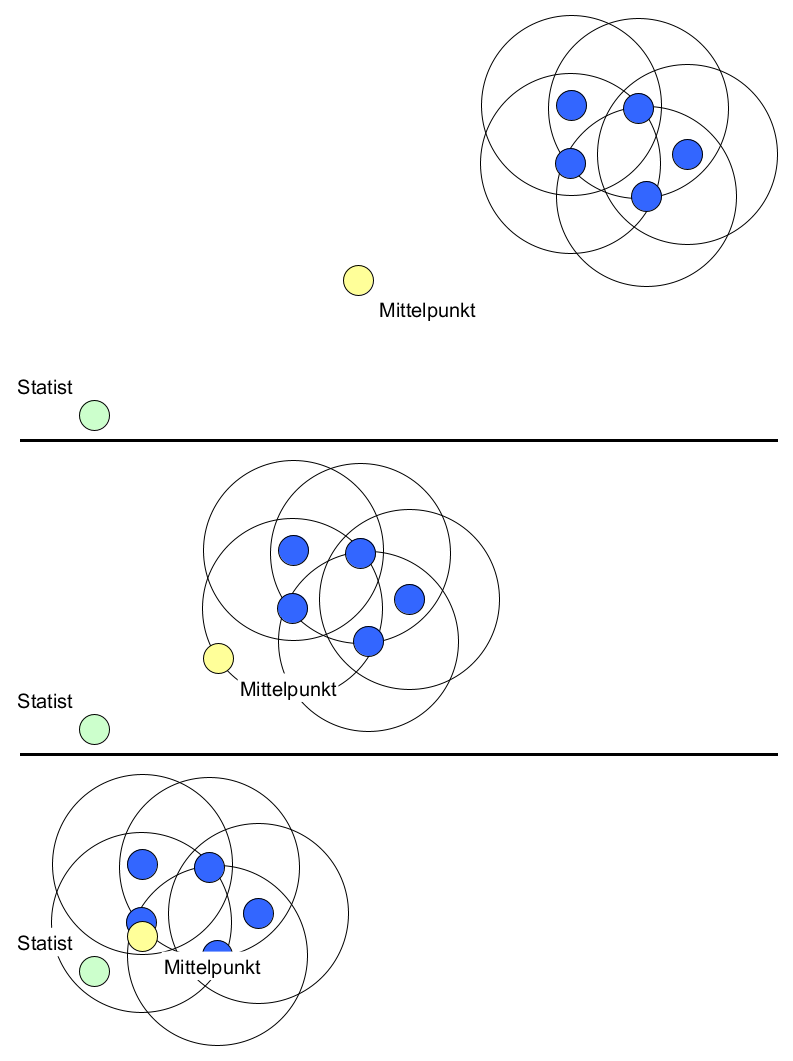
\includegraphics[width=\pictureWidthBig,keepaspectratio]{graphics/AlgorithmusStatist.png}
%	\caption{Funktionsweise des Statisten}
%	\label{pic:AlgorithmusStatist}
%\end{wrapfigure}

\begin{figure}[h]
	\centering
	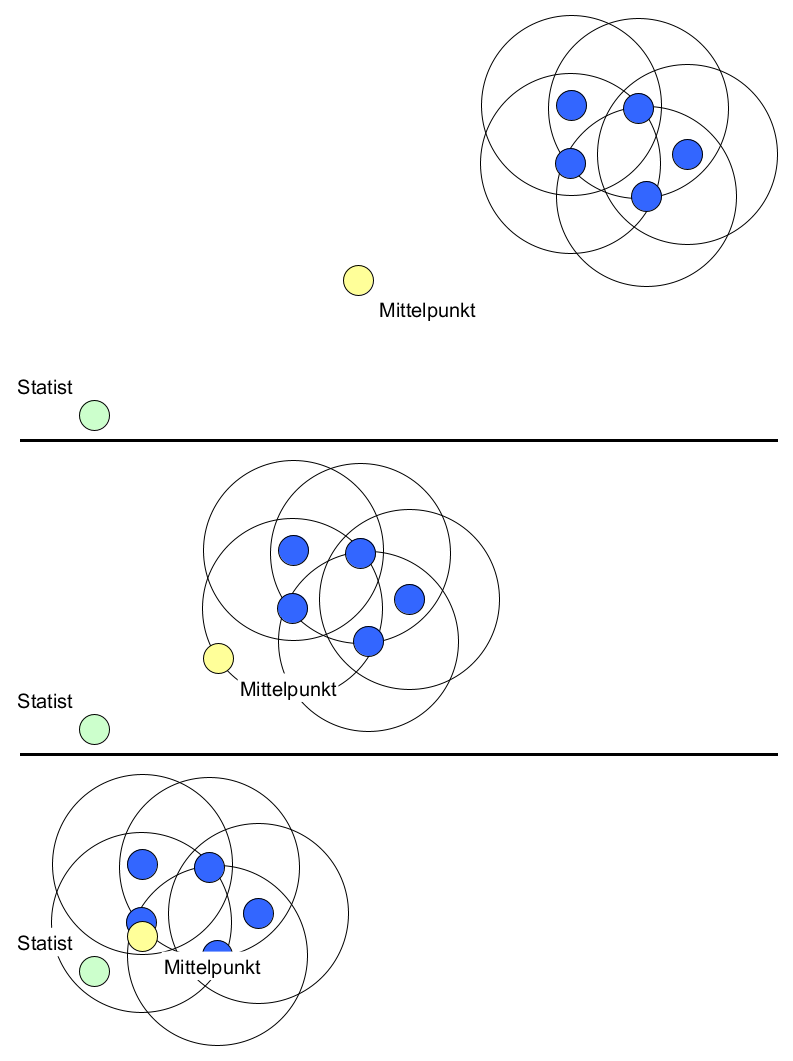
\includegraphics[width=0.6\textwidth,keepaspectratio]{graphics/AlgorithmusStatist.png}
	\caption{Funktionsweise des Statisten}
	\label{pic:AlgorithmusStatist}
\end{figure}

In \autoref{pic:AlgorithmusStatist} ist die Funktionsweise des Statisten dargestellt. Da der Statist nur dazu dient den Schwarmmittelpunkt zu verschieben, muss dieser kein physischer Roboter sein, sondern kann virtuell dargestellt werden. Dieser Statist kann auch das Stacking verwenden und somit seinen Effekt als Mittelpunkt-Verschieber vergrößern.

\subsubsection*{Der Statist als Node}

Der Statist ist leicht umzusetzen als \ac{ROS}-Node-Implementierung. Er muss nur irgendwo erstellt werden, bleibt dort stehen, sendet seine Positionsdaten einmalig an die anderen Roboter und wird letztlich wieder gelöscht werden, wenn er nicht mehr gebraucht wird. Da er sich nicht an anderen Robotern orientiert muss er selbst keine Topics abonnieren. Er selbst verbreitet auch nur seine Positionsdaten als einziges Topic. 

\paragraph*{Beispiel-Implementierung}
Aufgrund seiner Einfachheit kann der Statist leicht von anderen Robotern erstellt werden. Als Beispiel einer Implementierung würde sich ein einfaches Objekte mit Konstruktor und Destruktor realisieren lassen.

\begin{lstlisting}[style=cpp]
class Statist {
	public:
	Statist(int id, Position pos) {
		// send New_Robot.msg
		// send Position.msg
	}
	
	~Statist() {
		// send Delete\_Robot.msg
	}
};
\end{lstlisting}

Am Anfang der Funktion erstellt, die für die Abarbeitung eines Auftrags zuständig ist, wäre dieses Objekt quasi ein Selbstläufer der keinerlei Verwaltung brauchen würde.

\subsubsection*{Sonderregel für Statist}

Der Statist ist aber aus zweierlei Sicht eine Sonderregel im Schwarm. Zum einen muss er von den anderen Robotern auch dann beachtet werden, wenn er sich nicht innerhalb deren lokalen Reichweite befindet. Zum anderen arbeitet der Roboter nur mit seiner Position, nicht mit seiner Ausrichtung (da sich diese immer wieder anpassen müsste und es den Statisten wesentlich komplizierter gestalten würde). Aus diesem Grund muss der Statist als Roboter-Typ im Schwarm bekannt sein und seine Positionsdaten gesondert behandelt werden. Die Nachricht um einen neuen Roboter zu erstellen, würde also um einen Punkt erweitert werden, der eine Typzuordnung erlaubt.

\begin{lstlisting}[style=ros, title=Nachrichten-Typ: New\_Robot.msg]
uint8 robot_id			// Die ID des neuen Roboters
uint8 sub_id			// Die Sub-ID des Roboters
uint8 type				// Der Typ des Roboters
\end{lstlisting}

Damit ist der Schwarm physisch gesehen immer noch homogen, virtuell gesehen aber nicht mehr, da es nun einen Roboter-Typ gibt der nur virtuell auftreten kann.

\paragraph*{Vorteile gegenüber Anführern}
Der große Vorteil gegenüber der Steuerung des Schwarms mit Hilfe von Anführern ist, dass der Statist den Schwarm nicht aktiv lenken muss. Während ein Anführer den Schwarm mit seiner Ausrichtung aktiv beeinflussen muss, lenkt der Statist eher passiv, indem er den Schwarm zu sich kommen lässt. Dies braucht wesentlich weniger Ressourcen und ein Roboter braucht keine zweite Verhaltensweise.

\paragraph*{Nachteile gegenüber Anführern}
Auf der anderen Seite gibt es bei dieser Methode aber auch den Nachteile, dass sie einen zweiten Roboter-Typ einführt und damit erstmals die Grenze des homogenen Schwarms übertritt. Der neue Roboter-Typ braucht gesondertes Verhalten ihm gegenüber und er öffnet die Tür für weitere Roboter-Typen die den Schwarm nach und nach immer heterogener werden lassen.\\

\begin{wrapfigure}{r}{\pictureWidth}
	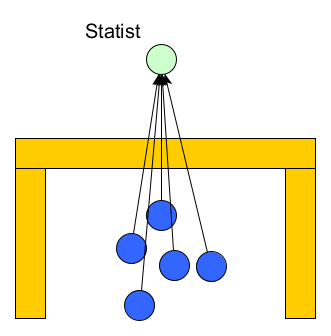
\includegraphics[width=\pictureWidth,keepaspectratio]{graphics/StatistSenke.png}
	\caption{Roboter stecken in einer Senke fest}
	\label{pic:StatistSenke}
\end{wrapfigure}

Letztlich wird das Verhalten mit einem Statisten aber ein anderes sein. Ist ein Anführer theoretisch noch in der Lage seinen Schwarm zu lenken, und damit auch um Hindernisse herum, kann ein Statist dies allgemein nicht. Der Schwärm würde in Richtung des Statisten wandern und Hindernissen auf dem Weg gegebenenfalls mit dem normalen Algorithmus ausweichen. Dabei könnte es vorkommen, dass sie in eine Senke getrieben werden und von selbst nicht mehr herauskommen (Veranschaulichung siehe \autoref{pic:StatistSenke}).

Andererseits könnte man mit mehreren Statisten, einem nach dem anderen, einen Weg abstecken dem die Roboter dann folgen. Es ließen sich also Etappen berechnen die die Roboter eine nach der anderen bewältigen müssen, wobei dies von einer zentralen Einheit gesteuert werden müsste. Die Auftragsvergabe oder eine andere Art von Anführer innerhalb des Schwarms wären dafür zuständig.


\subsection{Statisten als Auftragsvergabe}

Der Statist lässt sich nicht nur benutzen um einen Schwarm zu lenken. Mit seiner Besonderheit andere Roboter aus jeder Entfernung zu sich ziehen zu können, wäre es sehr interessant ihn zu benutzen um Roboter ihren Aufträgen zuzuteilen. Dies würde erfordern ihn von einer Auftragsvergabe-Node erstellen zu lassen, da diese Node noch einige weitere Aufgaben zu erledigen hätte.

\subsubsection*{Eine neue Herangehensweise an Aufträge}

Den Statisten zu benutzen um Aufträge zu 'verteilen' würde im Grunde genommen bedeuten, Aufträge nicht mehr zu verteilen. Stattdessen wird ein Statist dorthin gesetzt wo sich das Transportobjekt an seinem Aufnahmeort befindet.

Der gesamte Standby-Schwarm wird nun passiv in die Richtung des Statisten, und damit auch in Richtung des Transportobjektes, gelenkt. Übertritt nun ein Roboter die Grenze des Transportobjektes und befindet sich in seinem innere, wird ihm von der Node, die auch den Statisten hält, der Auftrag zugewiesen. Andere Roboter die folgen werden ebenfalls den Auftrag zugeteilt und die Roboter werden einen gesonderten Schwarm verschoben, genau wie es auch bei der vorigen Auftragsvergabe geschehen würde. Der Statist bleibt so lange aktiv bis sich so viele Roboter gefunden haben, wie es für den Auftrag erforderlich ist. Ist die erforderliche Zahl erreicht, wird die Vergabe-Node die Roboter mit einer \highlight{Freeze.msg} bewegungsunfähig machen und den Statisten mit der entsprechenden Nachricht löschen. Es befindet sich nun die geforderte Zahl an Robotern unterhalb des Transportobjektes und sie stehen still. Somit wurde wieder die gleiche Ausgangslage geschaffen, wie sie bei der vorigen Auftragsvergabe vorzufinden war, bevor der eigentliche Transport startete. Der Statist wurde wie ein Magnet dazu benutzt die Roboter einzusammeln die den Transport vollziehen sollen.
Nun hier an kann der Transport normal ablaufen. Entweder wird ein Anführer bestimmt der das Ziel kennt, und der eventuell virtuelle Kopien von sich erschafft, oder der Transport-Schwarm wird mit Hilfe eines zweiten Statisten an sein Ziel geführt.

Entgegen der normalen Auftragsvergabe, würde man die Roboter nicht von Anfang an zuweisen, sondern man würde den Statisten als eine Art Magnet nutzen um die Roboter aufzusammeln, die am schnellsten da sind. Man würde dadurch die Roboter bekommen die am nächsten dran sind oder schlicht schneller sind, als die anderen.

\paragraph*{Vorteile zur direkten Zuweisung}
Die Vorteile zur direkten Zuweisung liegen darin, dass die Roboter nicht von einem übergeordneten System ausgewählt werden müssen. Es braucht keine übergordnete Instanz die Roboter aussucht und dabei womöglich noch weitere Kriterien in Betracht ziehen muss wie Entfernung und eventuelle Unterschiede in der Geschwindigkeit der einzelnen Roboter. Die Lösung über einen Statisten ist nicht so streng wie über eine Sicherheitszone und passt sich gut in den Schwarm ein, es ist eine schöne, dynamische Lösung.

\paragraph*{Nachteile zu direkten Zuweisung}
Zusätzlich zu den Nachteilen die ein Statist selbst schon mitbringt, lässt sich die Geschwindigkeit anmerken. Ohne Tests lässt sich dies zwar nicht mit absoluter Sicherheit sagen, vermutlich wird die Variante mit einem Statisten aber langsamer sein als die Version mit der manuellen Zuordnung und einer Sicherheitszone. Der Grund hierfür ist schlicht, dass die Roboter die in die Sicherheitszone flüchten dies auf direktem Wege machen, wohingegen sich die Roboter nur grob an der Mitte des Schwarms ausrichten und der Statist dadurch nicht ansatzweise die selbe Wirkung hat wie eine Gefahrenzone.

\subsection{Ausschwärmen}

\autoref{subsec:EvaluationNegativerGruppendrang} hat bereits gezeigt, dass es mit Hilfe von negativem Gruppendrang möglich ist einen Schwarm ausschwärmen zu lassen und sich somit zu verteilen. Dies ist nützlich, damit die Roboter während des Standbys nicht im Weg anderer Roboter oder Menschen stehen.
Ein anderer Algorithmus wäre ebenfalls denkbar, der die Größe der Roboter langsam wachsen lässt.

\subsubsection*{Algorithmus}

\begin{wrapfigure}{r}{\pictureWidthSmall}
	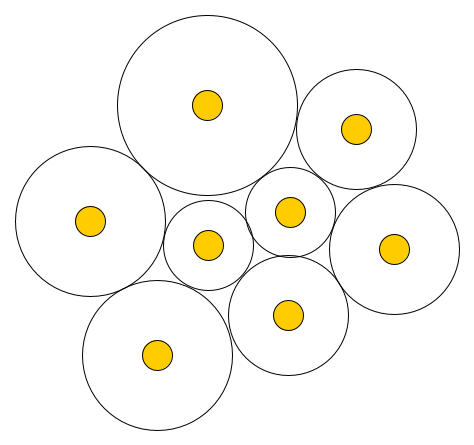
\includegraphics[width=\pictureWidthSmall,keepaspectratio]{graphics/LuftballonAlgorithmus.png}
	\caption{Der Luftballon-Algorithmus}
	\label{pic:Luftballon}
\end{wrapfigure}

Ähnlich wie bei einem Sack voll mit Luftballons, die alle gleichzeitig aufgepumpt werden würde sich die Größe der Roboter vergrößern. Dies geschieht so lange bis der 'aufgepumpte' Körper an mindestens 3 Punkten den eines anderen Roboters oder eine andere Grenze (beispielsweise ein Gefahrengebiet) berührt. Solange es nur weniger als drei Berührungspunkte gibt, wird der Körper wachsen und der Roboter durch seinen Fluchtreflex dafür sorgen wollen, dass er nicht weiter mit anderen Objekten kollidiert. Solange es nur weniger als drei Berührungspunkt gibt, wird es immer eine Seite geben, zu der er ausweichen kann. Trifft er auf den dritten Punkt ist er eingesperrt und seine Position befindet sich so weit weg von anderen Robotern wie nur möglich.

\subsubsection*{Umsetzung}
Für die Umsetzung müsste das generelle Verhalten der Roboter nicht angepasst werden. Das verteilen des Roboters geschieht durch den Fluchtreflex der bereits implementiert ist. Es müsste nur, ähnlich beim Stillstand über das \highlight{Freeze}-Kommando, eine kleine Routine im 'Unterbewusstsein' geschaffen werden, die die interne Größe immer weiter verändert bis der Roboter keinen Weg mehr sieht aus seiner Misere herauszukommen.

\subsubsection*{Nutzung für den Transport}
Auch im Transport wäre dieser Algorithmus nützlich. Finden sich die Roboter unter dem Transportobjekt ein, stehen sie still, sobald sie alle da sind. Der hier vorgestellte Algorithmus würde stattfinden, nachdem alle Roboter unter dem Transportobjekt sind. Sie würden ihre Größe anwachsen lassen und sich so möglichst gleichmäßig unterhalb des zu transportierenden Objektes verteilen. Die Grenzen der Sicherheitszone bilden dabei meist den dritten Berührungspunkt. Stehen alle Roboter still, braucht es theoretisch gesehen sogar nicht mal ein \highlight{Freeze}-Kommando, da sie sich aufgrund des beendeten Algorithmus nicht mehr weiter bewegen können dürften.
Sobald das Transportobjekt auf den Köpfen der Roboter abgesetzt ist, kann die Größe wieder auf den Normalzustand zurück schrumpfen und die Roboter beginnen damit den Transport umzusetzen.